\documentclass{article}
\usepackage[utf8]{inputenc}
\usepackage{graphicx}


\title{How to create a Voltage Divider with Gschem and Ngspice}
\author{Dylan Ortiz }

\date{March 29, 2020}

\begin{document}

\maketitle

\section{Get components}
Recognize the elements that will be required in order to build the voltage divider with the software Gschem.
\begin{center}
    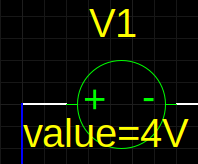
\includegraphics[width=.3\textwidth]{Vol.png}\\
    Voltage source\\
    
    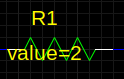
\includegraphics[width=.3\textwidth]{Res.png}\\
    Resistor 1 and 2\\
    
    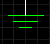
\includegraphics[width=.3\textwidth]{GRND.png}\\
    Ground\\
\end{center}
\section{Build voltage divider circuit}
After finding the elements needed for the circuit, we proceed to build the voltage divider, this means two resistors will be in series with a voltage source.
\begin{center}
    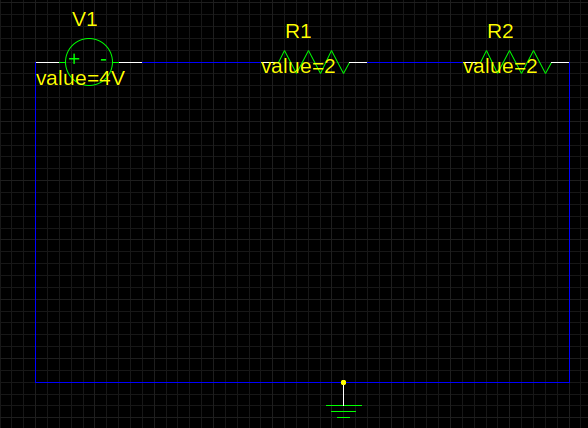
\includegraphics[width=.95\textwidth]{Voldiv.png}\\
    Voltage Divider
\end{center}
\section{Getting Values}
Once we have built our circuit we proceed to find the values of the voltage on each node by using Ngspice or gnetlist from the terminal.
\begin{center}
    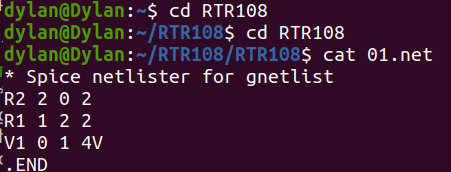
\includegraphics[width=.98\textwidth]{gnetlist.png}\\
    Values of voltage divider from Gnetlist.\\
    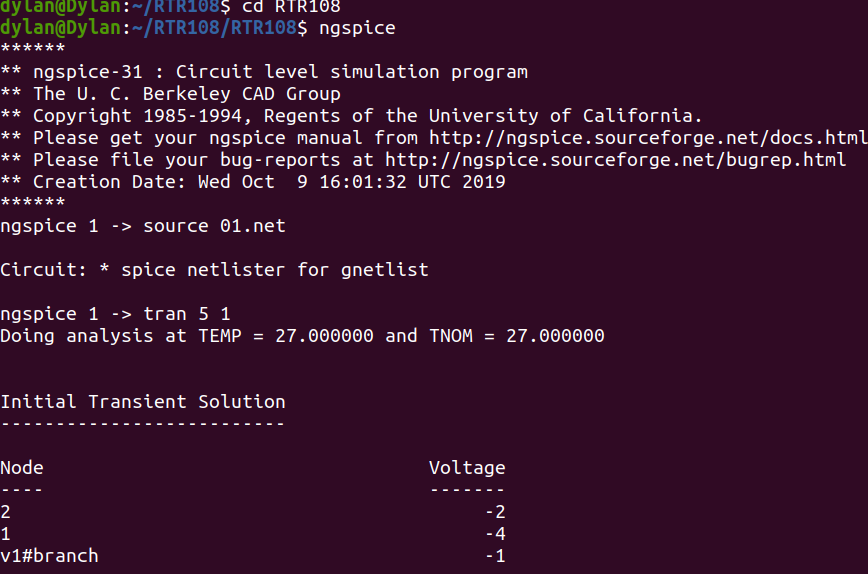
\includegraphics[width=.99\textwidth]{Ngspice.png}\\
    Values of voltage divider from Ngspice
\end{center}
\end{document}
